\section{Onyxia: an open source project to build cloud-native data science platforms}

The Onyxia project, initiated by the French Public Service and available at
onyxia.sh, is an open source project aimed at creating self-sufficient data science environments in the cloud or on-premises. This project can be seen as a “Platform as a Package” (PaaP) solution for organisations wishing to create a data science environment based on cloud technologies.

\subsection{Making cloud-technologies accessible to statisticians}

Our technology watch and literature review highlighted cloud-native technologies, in particular containerization and object storage, as instrumental in building a data science platform that is both scalable and flexible. Building on these insights, we established our initial on-premise Kubernetes cluster in 2020, integrating it with MinIO, an open-source object storage system designed to work seamlessly with Kubernetes. Yet, our first experiments highlighted a significant barrier to their widespread adoption: the complexity of their integration. This is an important consideration when building data architectures that prioritize modularity — an essential feature for the flexibility we aim to achieve. For instance, due to MinIO's compatibility with the Amazon S3 API, the storage source could easily be switched without requiring substantial modifications to one managed by a public cloud provider. However, modularity of the architecture components also entails that any data application launched on the cluster must be configured so as to communicate with all the components. For instance, in a big data setup, configuring Spark to operate on Kubernetes while interacting with datasets stored in MinIO requires an intricate set of configurations (specifying endpoints, access tokens, etc.), a skill set that typically lies beyond the expertise of statisticians.

This very insight is really the base of the Onyxia project : choosing technologies that foster autonomy won't actually foster autonomy if their complexity acts as a deterrent from widespread adoption in the structure. In recent years, statisticians at Insee already need to adapt to a changing environment in termes of their everyday tools : transitioning from proprietary software (SAS) to open-source ones (R, Python), acculturating to technologies that improve reproducibility (version control with Git), consuming and developing APIs, etc. These changes, that make their activity more and more akin to the one of software developers, already imply significant training and changes in the modalities of work everyday. In this regard, adoption of cloud-technologies was utterly dependent on making them readily accessible.

\begin{figure}[htbp]
    \centering
    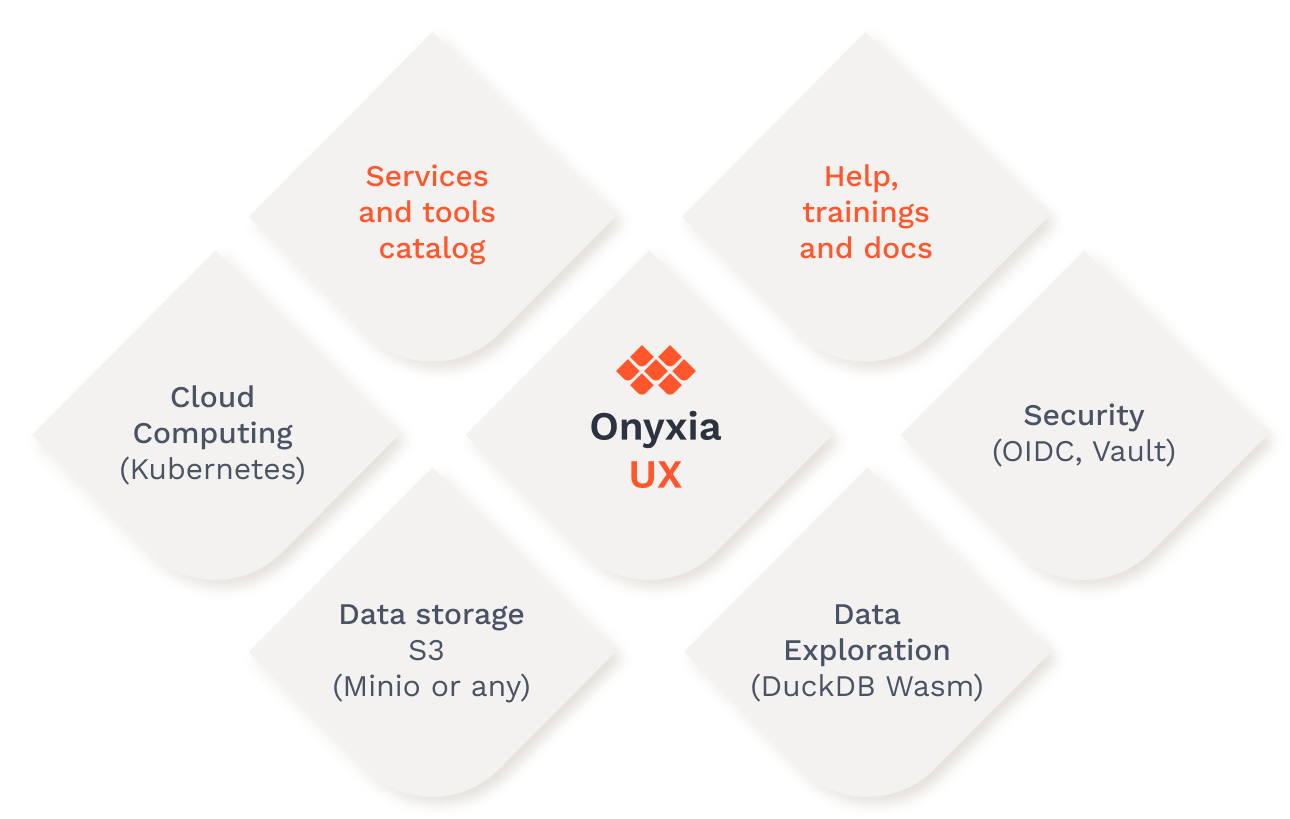
\includegraphics[width=\linewidth]{sections/img/onyxia-components.png}
    \caption{Onyxia is the technical binder between cloud-native modular components}
    \label{fig:onyxia-components}
\end{figure}

To bridge this gap, we developed Onyxia, an application that essentially acts as interface between the modular components that compose the architecture (see fig~\ref{fig:onyxia-components}). The main entrypoint of the user is a user-friendly web application\footnote{\url{https://github.com/InseeFrLab/onyxia-ui}} that enables users to launch services from a data science catalog (see section \ref{ssec:catalog}) as running containers on the underlying Kubernetes cluster. The interface between the UI and Kubernetes is done by a lightweight custom API\footnote{\url{https://github.com/InseeFrLab/onyxia-api}}, that essentially transforms the application request of the user into a set of manifests to deploy Kubernetes resources. For a given application, these resources are packaged under the form of Helm charts, a popular way of packaging potentially complex applications on Kubernetes \cite{gokhale2021creating}. Although users can configure a service to tailor it to their needs, they will most of the time just launch a service out-of-the-box and be able to start developing. This point really illustrates the added value of Onyxia in facilitating the adoption of cloud technologies. By injecting authentication information and configuration into the containers at the initialization, we ensure that users can launch and manage data science services in which they can interact seamlessly with the data from their bucket on MinIO, their sensitive information (tokens, passwords) stored in Vault, etc. This automatic injection, coupled with the pre-configuration of data science environments in Onyxia's catalogs of images\footnote{\url{https://github.com/InseeFrLab/images-datascience}} and associated helm-charts\footnote{\url{https://github.com/InseeFrLab/helm-charts-interactive-services}}, make it possible for users to execute potentially complex workloads - such as running distributed computations with Spark on Kubernetes using data stored in S3, or training deep-learning models using a GPU - without getting bogged down by the technicalities of configuration.

% TODO: figure : from launching a service to its deployment on Kube + S3, Vault ?

\subsection{Architectural choices aimed at fostering autonomy}
\label{ssec:principles}

The Onyxia project is based on a few structuring principles, with a central theme : fostering autonomy. First, at the level of the organization by preventing vendor lock-in. In order to get a competitive edge, many commercial cloud providers develop applications and protocols that customers need to use to access cloud resources but that are not interoperable, greatly complexifying potential migrations to another cloud platform \cite{opara2016critical}. Recognizing these challenges, there is a trend towards endorsing cloud-neutral strategies \cite{opara2017holistic} in order to reduce reliance on a single vendor’s specific solutions. In contrast, the use of Onyxia is inherently not restrictive: when an organization chooses to use it, it chooses the underlying technologies - containerization and object storage - but not the solution. The platform can be deployed on any Kubernetes cluster, either on-premise or in public clouds. Similarly, although Onyxia was designed to be used with MinIO because it is an open-source object-storage solution, but is also compatible with objects storage solutions from various cloud providers (AWS, GCP).

The other important level at which Onyxia fosters autonomy is at the level of users. Proprietary softwares that have been used intensively in official statistics - such as SAS or STATA - also produce a vendor lock-in phenomenon. The costs of licensing are high and can evolve quickly, and users are tied in certain ways of performing computations, preventing progressive upskilling. On the contrary, Onyxia aspires to be removable; we want to enhance users' familiarity and comfort with the underlying cloud technologies rather than act as a permanent fixture in their workflow. An illustrative example of this philosophy is the platform's approach to user actions: for tasks performed through the UI, such as launching a service or managing data, we provide users with the equivalent terminal commands, promoting a deeper understanding of what actually happens on the infrastructure when triggering something. Furthermore, all the services offered through Onyxia's catalog are open-source.

% TODO: figure show code

Naturally, the way Onyxia makes statisticians more autonomous in their work depends on their needs and familiarity with IT skills. Statisticians that just want to have access to extensive computational resources to experiment with new data sources or statistical methods will have access in a few clicks to easy-to-use, pre-configured data science environments, so that they can directly start to work and prototype their solution. However, many users want to go deeper and build actual prototypes of production applications for their projects: configuring initialization scripts to tailor the environments to their needs, deploying an interactive app that delivers data visualisation to users of their choice, deploying other services than those available in our catalogs, etc. For these advanced users to continue to push the boundaries of innovation, Onyxia gives them access to the underlying Kubernetes cluster. This means that users can freely open a terminal on an interactive service and interacts with the cluster - within the boundaries of their namespace - in order to apply custom resources and deploy custom applications or services.

Besides autonomy and scalability, the architectural choices of Onyxia also foster reproducibility of statistical computations. In the paradigm of containers, the user must learn to deal with resources which are by nature ephemeral, since they only exist at the time of their actual mobilization. This fosters the adoption of development best practices, notably the separation of the code — put on an internal or open-source forge such as GitLab or GitHub — the data — persisted on a specific storage solution, such as MinIO — and the computing environment. While this requires an entry cost for users, it also helps them to conceive their projects as pipelines, i.e. a series of sequential steps with well-defined inputs and outputs (akin to directed acyclic graph (DAG)). The projects developed in that manner are usually more reproducible and portable — they can work seamlessly on different computing environments — and thus also more readily shareable with peers.

% TODO: figure separation processes + DAG

\subsection{An extensive catalogue of services to cover the entire lifecycle of data science projects}
\label{ssec:catalog}

In developing the Onyxia platform, our intention was to provide statisticians with a comprehensive environment designed to support the prototyping of their data science projects from start to finish. As depicted in Figure~\ref{fig:onyxia-catalog}, the platform offers a vast array of services that span the complete lifecycle of a data science project.

\begin{figure}[htbp]
    \centering
    \makebox[\textwidth][c]{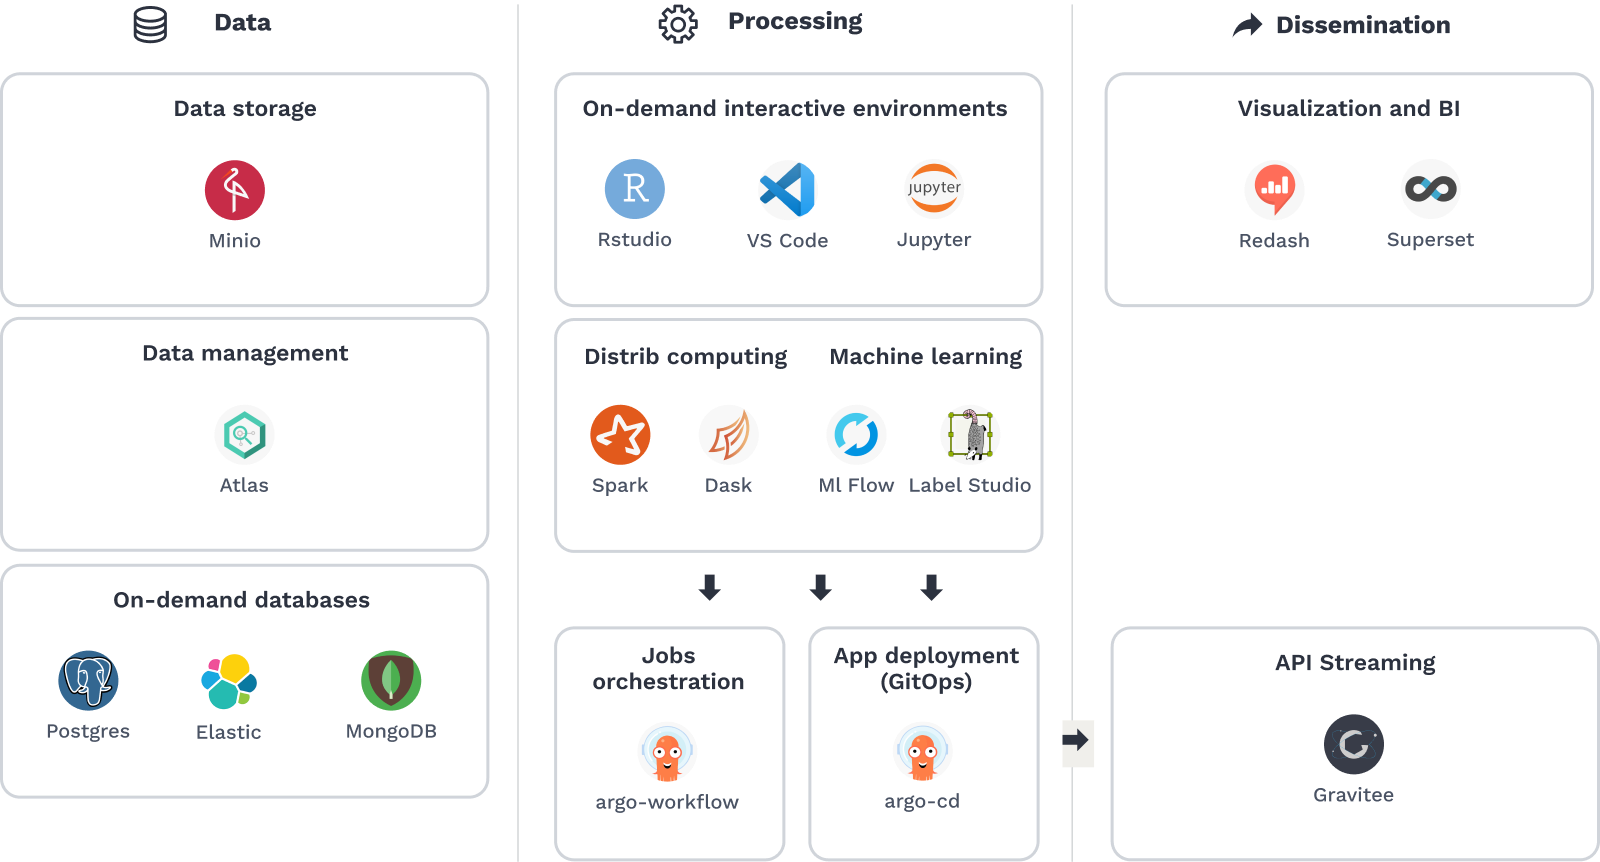
\includegraphics[width=1.2\textwidth]{sections/img/onyxia-catalog.png}}
    \caption{Onyxia's catalog aims at covering the entire lifecycle of data science projects}
    \label{fig:onyxia-catalog}
\end{figure}

The primary usage of the platform is the deployment of interactive development environments (IDE), such as RStudio, Jupyter, or VSCode. These IDEs come equipped with the latest kernels of major open-source programming languages commonly employed by public statisticians (R, Python, Julia), as well as an extensive collection of packages commonly used in data science for each language. In order to ensure that services remain up-to-date and consistent between them, we maintain our own stack of underlying Docker images and rebuilt it weekly. The stack of image is fully open-source and can thus be reused outside of Onyxia\footnote{\url{https://github.com/InseeFrLab/images-datascience}}.

As discussed in previous sections, the persistence layer of these interactive environments is mainly carried out by MinIO, Onyxia's default object storage solution. As it is based on a standardized REST API, files can be easily queried directly from R or Python using high-level packages. This in itself is an important step of ensuring reproducibility: the input files of a project are not mounted manually and then specified via paths adherent to a specific infrastructure and filesystem. Rather, files are specified as HTTP queries, making the overall structure of projects much more extendable. In our experience, the object-storage paradigm covers very well the needs of most statistical projects we accompany. However, additional database services such as PostgreSQL and MongoDB are available for applications with specific needs, such as those requiring online transaction processing (OLTP) capabilities or document-oriented storage.

As Onyxia was developed to allow experimentation with big data sources and machine learning methods, we also provide services optimized for scalability. For instance, frameworks like Spark and Trino that enable to perform distributed computations within Kubernetes. These services come pre-configured to integrate seamlessly with S3 storage, thus facilitating building integrated and efficient data pipelines.

Beyond mere experimentation, our goal is to empower statisticians to transition from trial phases to production-ready projects. In lines with principles from the DevOps approach, this involves facilitating the deployment of prototypes and their continuous improvement over time. To this end, we provide a set of open-source tools aimed at automatizing and industrializing the process of deploying data-intensive applications (ArgoCD, Argo-Workflows, MLFlow). For projects leveraging machine-learning models, statisticians can serve their models through APIs, deploy them using the aforementioned tools, and and manage their lifecycle using an API manager such as Gravitee. Section~\ref{sec:mlops} will delve into how these tools, particularly MLFlow, have been instrumental in putting machine learning models in production at Insee, in accordance with MLOps principles.

In section~\ref{ssec:principles}, we stressed that one of Onyxia's fundamental design principle was to avoid vendor lock-in. In line with this idea, organizations that implement Onyxia are at liberty to customize catalogs to suit their specific requirements, or even opt to construct their own catalogs independent of Onyxia's default offerings. This flexibility ensures that organizations are not confined to a single solution or provider, and can adapt the platform to their evolving needs.

\subsection{Building commons : an open-source project and an open-innovation platform}

As a fully open-source initiative, the Onyxia project aims at building "knowledge commons" by promoting and building software that can be easily reused in official statistics and beyond \cite{schweik2006free}. This concerns first of all the components on which Onyxia are based: both its constitutive technological bricks (Kubernetes, MinIO, Vault) as well as all the services from the catalog are open-source. But more crucially, all the code of the project is available openly on GitHub\footnote{\url{https://github.com/InseeFrLab/onyxia}}. Alongside an in-depth documentation\footnote{\url{https://docs.onyxia.sh/}}, this greatly facilitates the potential for other organizations to create instances of data science platforms built upon the Onyxia software and thus the principles it promotes. This enabled the project to attract a growing community of contributors from official statistics (Statistics Norway), NGOs (Mercator Ocean), research centres and even industry, thus transitioning progressively towards a more decentralized governance of the project. In the next years, the involvement of NSIs from the European Statistical System is expected to grow as Onyxia was chosen as the reference data science platform in the context of the One-Stop-Shop for Artificial Intelligence/Machine Learning for Official Statistics (AIML4OS).



- SSP CLoud
- Orientation plateforme : instance vivante d'Onyxia, ouverte, collaborative, sandbox (cf. ref papier SSP Cloud sur l'aspect plateforme)
- Innovation ouverte $\rightarrow$ littérature
- Open-data
- Instance de partage : formations reproductibles + utilisation dans les écoles de stats + hackathons (organisation annuelle du funathon cf. one-stop-shop)
